\documentclass[a4paper,10pt]{article}

\usepackage[brazilian]{babel}
\usepackage[utf8]{inputenc}
\usepackage{titlesec}
\usepackage{graphicx}
\usepackage{mathtools}
\usepackage{amsthm}
\usepackage{amsfonts}
\usepackage[top=1.0in,bottom=1.0in]{geometry}
\usepackage{hyperref}
\usepackage[singlelinecheck=false]{caption}
\usepackage[backend=biber,url=true,doi=true,eprint=false,style=alphabetic]{biblatex}
\usepackage{enumitem}
\usepackage[x11names, rgb]{xcolor}
\usepackage{tikz}
\usepackage[justification=centering]{caption}
\usepackage{indentfirst}
\usetikzlibrary{snakes,arrows,shapes}

\addbibresource{../reports/common/references.bib}

\newcommand\blfootnote[1]{%
  \begingroup
  \renewcommand\thefootnote{}\footnote{#1}%
  \addtocounter{footnote}{-1}%
  \endgroup
}

\DeclareMathOperator*{\argmin}{arg\,min}
\DeclareMathOperator*{\argmax}{arg\,max}

\newcommand\defeq{\mathrel{\overset{\makebox[0pt]{\mbox{\normalfont\tiny\sffamily def}}}{=}}}

\titleformat{\section}
  {\normalfont\scshape\bfseries}{\thesection}{1em}{}
\titleformat{\subsection}
  {\normalfont\scshape\bfseries}{\thesubsection}{1em}{}
\titleformat{\paragraph}
  {\normalfont}{\theparagraph}{1em}{}
\titleformat{\subparagraph}
  {\normalfont}{\thesubparagraph}{1em}{}

\captionsetup[table]{labelsep=space}

\theoremstyle{plain}

\newtheorem*{spn-def}{Definição}
\newtheorem*{spn-thm}{Teorema}

\setlength{\parskip}{1em}

\title{\textbf{Aprendizado Automático de Sum-Product Networks (SPNs)}}

\begin{document}
\date{}
\author{}
\vspace*{-40pt}
{\let\newpage\relax\maketitle}

Aluno: Renato Lui Geh (Bacharelado em Ciência da Computação)

Orientador: Denis Deratani Mauá (IME-USP)

\section{Introdução}

O objetivo deste projeto de Iniciação Científica é utilizar Aprendizado de Máquina para aprender
automaticamente a estrutura de um modelo probabilístico denominado Sum-Product Network (SPN).

Modelos probabilísticos baseados em grafos (PGM) têm como objetivo representar distribuições de
probabilidade de forma compacta.

Para extrair conhecimento de um modelo probabilístico, computa-se inferência. Inferência na
maioria dos modelos gráficos é intratável, já que o número de termos na distribuição é exponencial.

Existem modelos gráficos que possuem inferência tratável, porém a maioria não consegue representar
de forma compacta e geral uma distribuição. A maioria dos PGMs solucionam o problema da
intractabilidade computando a inferência aproximada.

Sum-Product Networks são PGMs que, quando completas e consistentes, computam a inferência exata e
em tempo tratável. Adicionalmente, SPNs se mostraram mais gerais que outros modelos que computam
inferência em tempo tratável.\cite{poon-domingos}

Como aprendizado de uma SPN depende da inferência, a intractabilidade do aprendizado depende da
intractabilidade da inferência.

\section{Definição}

Esta seção faz uma breve descrição de Sum-Product Networks, assim como explica quais são os
desafios e problemas relacionados à SPNs.

\subsection{Modelos Gráficos Probabilísticos (PGM)}

Um modelo probabilístico tem como objetivo representar uma distribuição de probabilidade de forma
compacta. PGMs são utilizadas em \textit{data mining}, previsão de eventos, classificação, entre
outros.

Para fazer previsões, deduzir eventos ou extrair novo conhecimento, faz-se inferência na
distribuição de probabilidade. Inferência pode ser vista como uma probabilidade de um certo evento
ocorrer dados os eventos observados:

\begin{equation*}
  P(X=x_1,\ldots,x_n|\mathbf{e}=e_1,\ldots,e_q)
\end{equation*}

O conjunto $X=\{x_1,\ldots,x_n\}$ representa a \textit{query}, ou seja, o evento que deve ser
inferido. O conjunto $\mathbf{e}=\{e_1,\ldots,e_q\}$ é dito a evidência, as variáveis que já são
conhecidas. Probabilidades do tipo $P(a|b)$ são chamadas de probabilidades posteriores.

Para representar uma distribuição de probabilidade, é preciso tomar as probabilidades de cada
possível evento. Por exemplo, sejam duas variáveis $A$ e $B$ cujos possíveis valores são Booleanos,
e $B$ depende de $A$, então pode-se montar as seguintes tabelas:

\begin{table}[h]
  \begin{center}
    \begin{tabular}{l | c | c}
      & $P(A)$ & $P(B)$ \\
      \hline
      $1$ & $P(A=1)=0.4=\theta_a$ & $P(B=1)=0.8=\theta_b$ \\
      $0$ & $P(A=0)=0.6=\theta_{\overline{a}}$ & $P(B=0)=0.2=\theta_{\overline{b}}$ \\
    \end{tabular}
    \newline
    \vspace*{0.5cm}
    \newline
    \begin{tabular}{l | c | c}
      & $A=0$ & $A=1$ \\
      \hline
      $B=1$ & $P(B=1|A=0)=0.3=\theta_{b|\overline{a}}$ & $P(B=1|A=1)=0.4=\theta_{b|a}$ \\
      $B=0$ & $P(B=0|A=0)=0.7=\theta_{\overline{b}|\overline{a}}$ & $P(B=0|A=1)=0.6=\theta_{\overline{b}|a}$ \\
    \end{tabular}
  \end{center}
\end{table}

Pela definição de probabilidade condicional,

\begin{equation*}
  P(X, Y) = P(X)P(Y|X)
\end{equation*}

chega-se à distribuição de probabilidade das variáveis $A$ e $B$:

\begin{table}[h]
  \begin{center}
    \begin{tabular}{c c | c}
      $A$ & $B$ & $P(A, B)$ \\
      \hline
      $0$ & $0$ & $\theta_{\overline{a}}\theta_{\overline{b}|\overline{a}}$ \\
      $0$ & $1$ & $\theta_{\overline{a}}\theta_{b|\overline{a}}$ \\
      $1$ & $0$ & $\theta_a\theta_{\overline{b}|a}$ \\
      $1$ & $1$ & $\theta_a\theta_{a|b}$ \\
    \end{tabular}
  \end{center}
\end{table}

É fácil notar que dado um número $n$ de variáveis, as possíveis probabilidades são $n^2$. $O(n^2)$
é intratável, e portanto é necessário representar distribuições de forma compacta e computar
inferência em tempo tratável.

Redes Bayesianas conseguem representar distribuições de probabilidade, porém inferência no caso
geral é intratável, e portanto recorrem a inferência aproximada. Outros modelos, como mixture
models e árvores thin junction possuem inferência tratável, porém são limitadas a certas
distribuições. Portanto, um modelo cuja inferência seja tratável e que possa representar uma grande
variedade de distribuições é desejável.

\subsection{Sum-Product Networks}

Em 2011, foi proposta\cite{poon-domingos} uma nova classe de PGM chamada Sum-Product Network.

SPNs, quando completas e consistentes, têm inferência exata e tratável. Representam compactamente
uma distribuição de probabilidade e se mostraram mais gerais do que outros modelos com inferência
tratável.

SPNs representam uma distribuição de probabilidade por meio de uma função polinomial denominada
\textit{network polynomial} \cite{bayes-net-darwiche, poon-domingos}. Tomando o exemplo da
subseção passada, a network polynomial resultante é dada por:

\begin{equation*}
  f = \lambda_a\lambda_b\theta_a\theta_{b|a} +
  \lambda_a\lambda_{\overline{b}}\theta_a\theta_{\overline{b}|a} +
  \lambda_{\overline{a}}\lambda_b\theta_{\overline{a}}\theta_{b|\overline{a}} +
  \lambda_{\overline{a}}\lambda_{\overline{b}}\theta_{\overline{a}}\theta_{\overline{b}|\overline{a}}
\end{equation*}

Onde $\lambda_{a}$ é o indicador da variável $A$ e toma valores consistentes à evidência dada.

\begin{figure}[h]
  \centering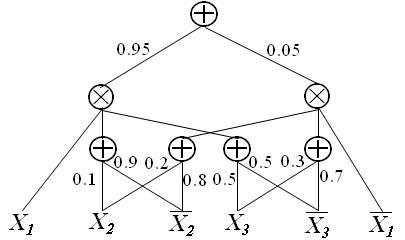
\includegraphics[scale=0.7]{imgs/domingos_poon.jpg}
  \caption{Uma SPN com variáveis Booleanas, onde $x_1,\ldots,x_d$ e $\overline{x}_1,\ldots,
    \overline{x}_d$ são folhas e o resto dos nós são somas ou produtos.\cite{poon-domingos}}
\end{figure}

Uma SPN é representada por um dígrafo acíclico onde as folhas são distribuições monovariáveis, ou
seja, representam uma das variáveis; e cada camada de nó interno é alternado entre um nó soma e nó
produto. Toda aresta que parte de um nó qualquer para um nó soma possue um peso não negativo.

O valor de uma SPN é o valor do nó raíz. O valor de um nó variável é a distribuição da própria
variável. O valor de um nó soma é a soma ponderada dos nós filhos dela. O valor de um nó produto
é o produto dos filhos.

Estudos em aprendizado de SPNs mostraram grande potencial. Em~\cite{poon-domingos}, Poon e Domingos
mostraram, por meio de experimentos, que SPNs tiveram melhor desempenho que outros modelos. Nesse
trabalho, o aprendizado foi realizado com uma estrutura já existente (e portanto menos flexível),
apenas aprendendo os pesos. Em~\cite{gens-domingos}, Gens e Domingos mostraram que, por meio do
aprendizado da estrutura e dos pesos, é possível gerar uma SPN ainda mais geral.

\section{Aplicações}

SPNs obtiveram resultados impressionantes em muitos conjuntos de dados\cite{website:spn-uwashington}, tais como:

\begin{itemize} \itemsep0pt
  \item Reconstrução de imagens.
  \item Classificação.
  \item Reconhecimento de atividade.
  \item Logs click-through.
  \item Sequências de ácido nucleico.
  \item Filtragem colaborativa.
\end{itemize}


\section{Objetivos}

Neste projeto de Iniciação Científica, o aluno irá estudar os seguintes tópicos:

\begin{itemize}
  \item Propriedades e estrutura de uma Sum-Product Network.
  \item Inferência em SPNs.
  \item Aprendizado:
  \begin{itemize}
    \item Dos pesos de uma SPN.\cite{poon-domingos}
    \item Da estrutura de uma SPN.\cite{gens-domingos}
    \item Por busca gulosa.\cite{greedy-search}
    \item Por clustering de variáveis.\cite{clustering}
    \item Por SPNs bayesianas não-paramétricas.\cite{non-parametric-bayesian}
  \end{itemize}
\end{itemize}

\section{Cronograma}

O aluno deverá reservar 10 horas por semana para estudos relacionados ao projeto. Além disso, o
aluno irá escrever relatórios semanais do que foi estudado na semana. Os relatórios estarão 
disponíveis em:

\subparagraph{\url{http://www.ime.usp.br/~renatolg/spn/doc/reports/}}

Tanto os relatórios quanto as implementações estarão disponíveis pelo repositório do projeto:

\subparagraph{\url{https://github.com/RenatoGeh/spn/}}

\newpage

\printbibliography

\end{document}
